% Eric Gullufsen - OSU Networking Course - Spring 2015
% Lab 1
\documentclass[12pt]{article}
\usepackage{amsmath}
\usepackage{amsfonts}
\usepackage{amsthm}
% need to include .png screenshots
\usepackage{graphicx}
\usepackage{verbatim}
\begin{document}
\title{CS 372 - Introduction to Computer Networks - Lab 1}
\author{Eric Gullufsen}
\date{9 April 2016}
\maketitle

\section{Problems 1 - 6}
\begin{enumerate}

\item
List 3 different protocols that appear in the protocol column in the unfiltered packet-listing 
window in step 7 above.\\
\textit{Answer}: In the figure 2 below we can see (among others) the TCP, HTTP, and DNS protocols.

\item
How long did it take from when the HTTP GET message was sent until the HTTP OK reply
was received?\\
\textit{Answer}: As the lab instructions suggest, we switch the Time display format
and find (see figure 3 below) that the bit of math we must perform is 
$0.848417 - 0.73364 = 0.114777$ seconds.

\item
What is the Internet address of the gaia.cs.umass.edu?
What is the Internet address of your computer?\\
\textit{Answer}: From any of the figures included below, we can see that
the IP address of the destination host is $128.119.245.12$.

\item
Print the two HTTP messages (GET and OK referred to in question 2 above.
To do so, select \textit{Print} from the Wireshark \textit{File} command menu,
and select the \textit{"Selected Packet Only"} and \textit{"Print as displayed"}
radial buttons, and then click OK.\\
\textit{Answer}: It's a bit cumbersome, but I've included the .txt files output
by wireshark, instead of printing them to a physical printer. First is the GET
request sent from my computer to the umass server, second is the reply info.\\

\tiny
\verbatiminput{lab1_wiresharkinfo.out}
\normalsize

\tiny
\verbatiminput{lab1_wiresharkinfo_OK.out}
\normalsize


\end{enumerate}

%comment timez!!!!!!!!!!!!!!!

% figure 1
\begin{figure}[ht]
\centering
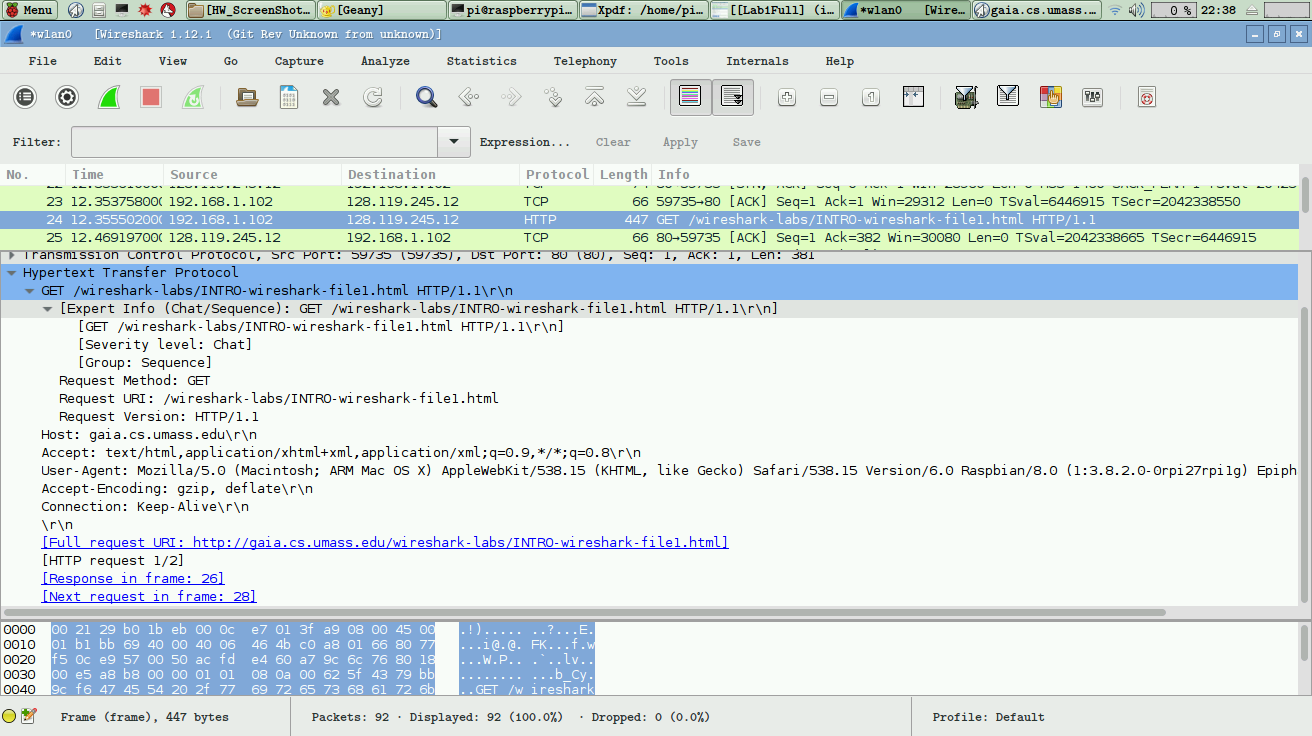
\includegraphics[scale=0.2]{Lab1Fullv2.png}
\caption{Showing complete HTTP protocol info for request}
\end{figure}

% figure 2
\begin{figure}[ht]
\centering
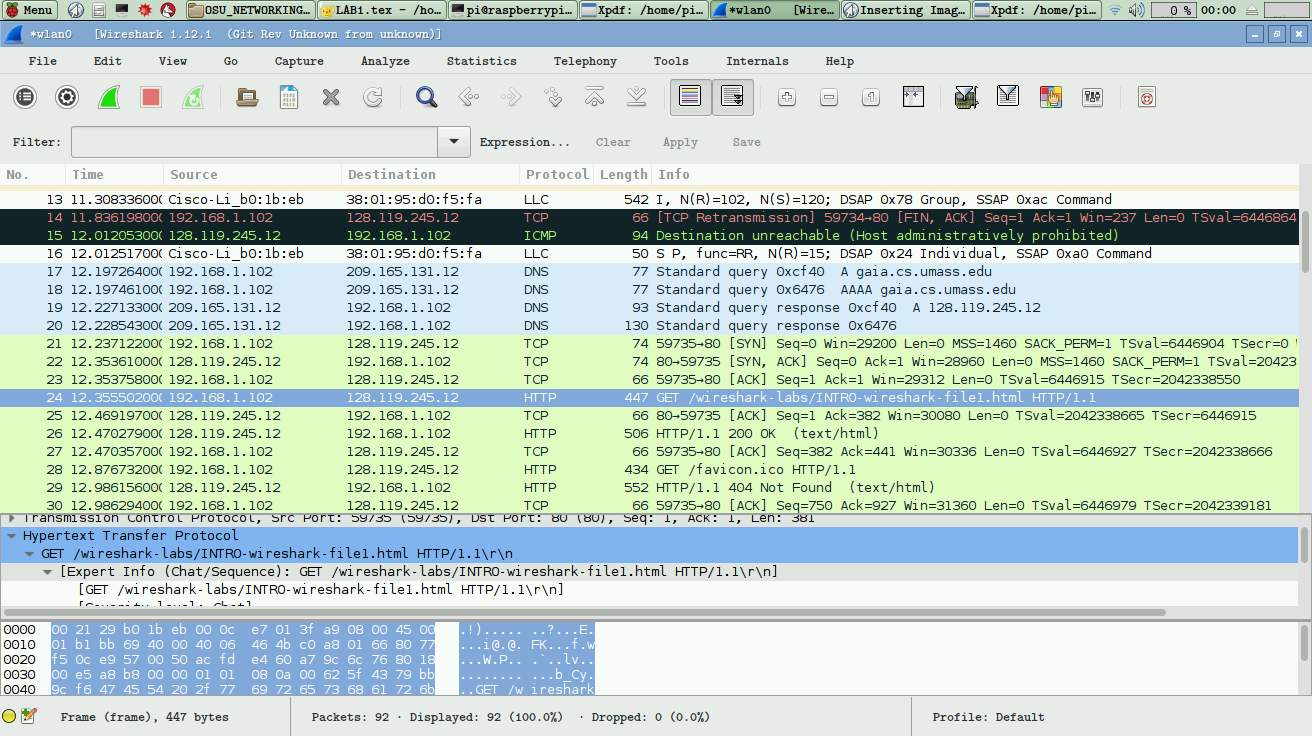
\includegraphics[scale=0.2]{Lab1Protocols.png}
\caption{Three (plus) different protocols listed}
\end{figure}

% figure 3
\begin{figure}[ht]
\centering
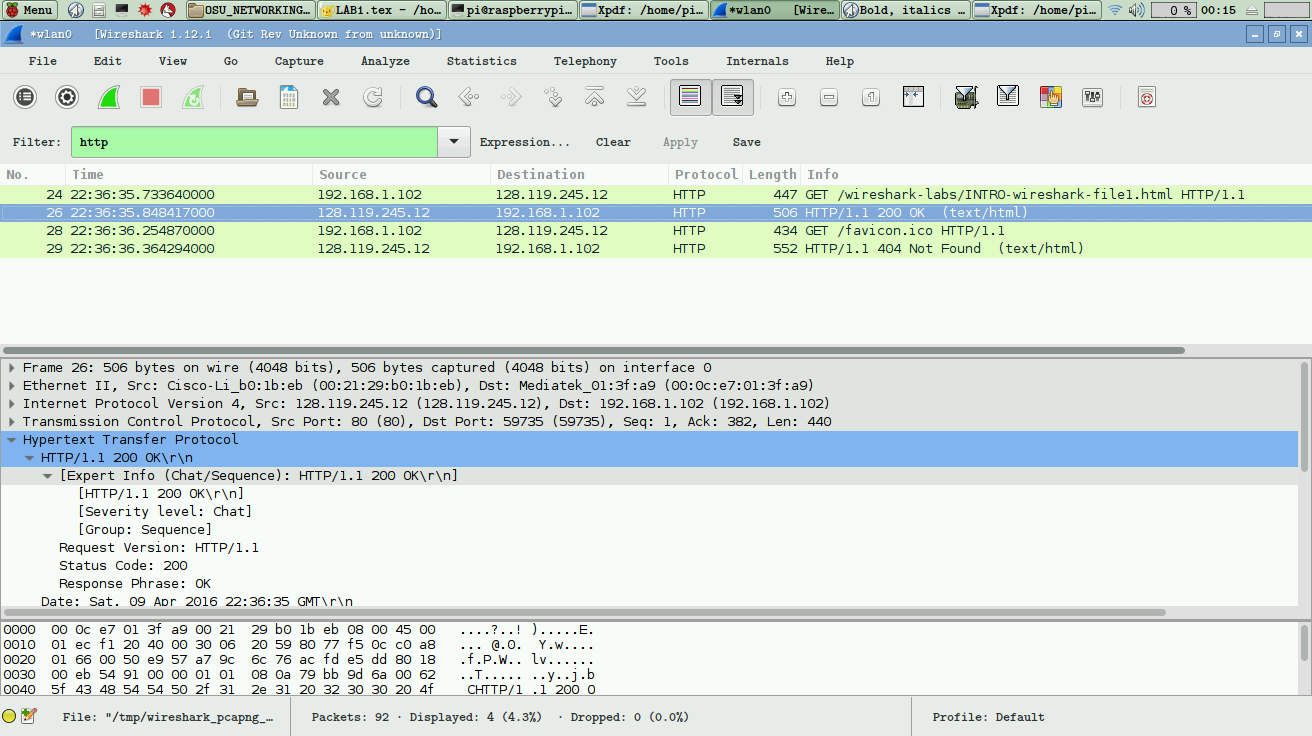
\includegraphics[scale=0.2]{Lab1Time.png}
\caption{Time display changed to Time-of-Day for calculation.}
\end{figure}

\end{document}
